\documentclass[../BTL.tex]{subfiles}
\begin{document}

\section{Phân tích và thiết kế hệ thống}
\subsection{Biểu đồ phân cấp chức năng (BFD - Bussiness Function Diagram)}
Biểu đồ ERD được vẽ như trên hình \ref{fig:BFD_LTW}.
\begin{figure}
    \centering
    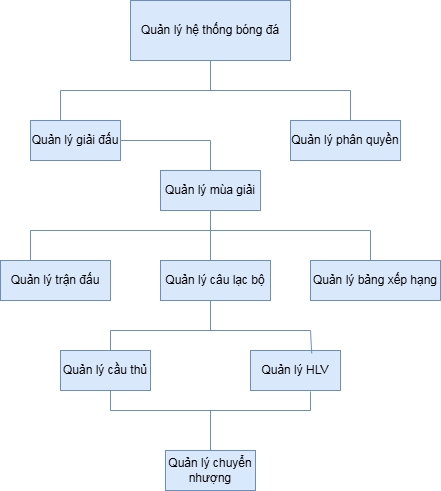
\includegraphics[width=0.8\linewidth]{Hinhve/BFD_LTW.png}
    \caption{Biểu đồ phân cấp chức năng}
    \label{fig:BFD_LTW}
\end{figure}
\subsection{Biểu đồ luồng dữ liệu (DFD - Data Flow Diagram)}
Biểu đồ DFD được vẽ như trên hình
 \ref{fig:DFDV2_LTW}.
\begin{figure}
    \centering
    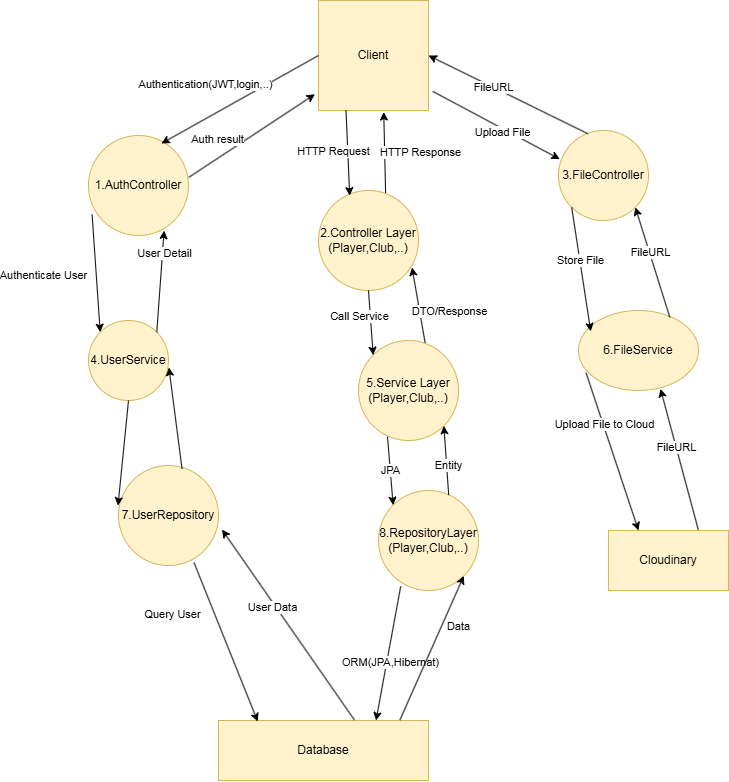
\includegraphics[width=1\linewidth]{Hinhve/DFDV2_LTW.png}
    \caption{Biểu đồ luồng dữ liệu}
    \label{fig:DFDV2_LTW}
\end{figure}
\section{Cơ sở dữ liệu}
\subsection{Giới thiệu}
MySQL là một hệ quản trị cơ sở dữ liệu mã nguồn mở (RDBMS) phổ biến, được phát triển bởi Oracle Corporation. MySQL sử dụng ngôn ngữ truy vấn có cấu trúc (SQL) để quản lý và thao tác dữ liệu. Một số đặc điểm nổi bật của MySQL bao gồm:

\begin{itemize}
    \item Hiệu suất cao: MySQL được tối ưu hóa cho tốc độ và hiệu suất, cho phép xử lý các truy vấn lớn một cách nhanh chóng.
    \item Độ tin cậy: MySQL cung cấp các tính năng như sao lưu và phục hồi, đảm bảo an toàn cho dữ liệu.
    \item Hỗ trợ giao dịch: MySQL hỗ trợ các giao dịch ACID (Atomicity, Consistency, Isolation, Durability), giúp đảm bảo tính toàn vẹn của dữ liệu.
    \item Khả năng mở rộng: MySQL có thể mở rộng để xử lý khối lượng dữ liệu lớn và nhiều người dùng đồng thời.
    \item Cộng đồng lớn: Là một trong những RDBMS phổ biến nhất, MySQL có một cộng đồng lớn và nhiều tài liệu hỗ trợ.
\end{itemize}
\subsection{ Kiến thức áp dụng}
Trong BTL này, nhóm em đã vận dụng hiệu quả các kiến thức về quản trị cơ sở dữ liệu MySQL. Chúng em đã thực hành các thao tác cơ bản như tạo cơ sở dữ liệu, thiết kế và tạo bảng với cấu trúc phù hợp cho ứng dụng web thể thao. Đặc biệt, nhóm đã triển khai thành công các khóa chính phức hợp (composite keys) trên một số bảng quan hệ, giúp đảm bảo tính toàn vẹn dữ liệu. Ngoài ra, nhóm đã thực hiện thành thạo các thao tác thêm, đọc, sửa, xóa dữ liệu thông qua các câu lệnh SQL, tạo nền tảng dữ liệu vững chắc cho ứng dụng.
\section{Ngôn ngữ lập trình}
\subsection{Java}
\subsubsection{Giới thiệu}
Java là một ngôn ngữ lập trình hướng đối tượng, được phát triển bởi Sun Microsystems (hiện nay thuộc Oracle Corporation) vào giữa những năm 1990. Java được thiết kế với mục tiêu "viết một lần, chạy mọi nơi" (WORA), có nghĩa là mã nguồn Java có thể chạy trên bất kỳ nền tảng nào có cài đặt Java Virtual Machine (JVM). Một số đặc điểm nổi bật của Java bao gồm:

\begin{itemize}
    \item Hướng đối tượng: Java hỗ trợ các nguyên tắc lập trình hướng đối tượng như kế thừa, đa hình, và đóng gói, giúp tổ chức mã nguồn một cách hiệu quả và dễ bảo trì.
    \item Độc lập nền tảng: Nhờ vào JVM, mã Java có thể chạy trên nhiều hệ điều hành khác nhau mà không cần thay đổi.
    \item Quản lý bộ nhớ tự động: Java sử dụng Garbage Collection để tự động quản lý bộ nhớ, giúp giảm thiểu rủi ro rò rỉ bộ nhớ.
    \item Thư viện phong phú: Java cung cấp một bộ thư viện lớn (Java Standard Library) hỗ trợ nhiều chức năng từ xử lý chuỗi, nhập/xuất, đến lập trình mạng và giao diện người dùng.
    \item Bảo mật: Java có nhiều tính năng bảo mật tích hợp, giúp bảo vệ ứng dụng khỏi các mối đe dọa.
\end{itemize}
\subsubsection{Kiến thức áp dụng }
Khi phát triển phần backend của ứng dụng, nhóm em đã áp dụng sâu rộng kiến thức về ngôn ngữ Java. Chúng em đã vận dụng hiệu quả các cấu trúc dữ liệu Collections để quản lý và xử lý dữ liệu động. Các nguyên lý lập trình hướng đối tượng đã được triển khai xuyên suốt, với việc áp dụng tính đóng gói để bảo vệ dữ liệu, tận dụng kế thừa để tái sử dụng mã nguồn, ứng dụng đa hình để xử lý linh hoạt các đối tượng khác nhau, và áp dụng tính trừu tượng để đơn giản hóa mô hình dữ liệu phức tạp. Những nguyên lý này đã giúp nhóm xây dựng một hệ thống backend có khả năng bảo trì cao.
\subsection{Javascript}
\subsubsection{ Giới thiệu}
JavaScript viết tắt là JS là ngôn ngữ lập trình bậc cao phổ biến dùng để tạo ra các trang web tương tác, được tích hợp và nhúng vào HTML giúp website trở nên sống động hơn. JavaScript đóng vai trò như một phần của trang web, thực thi cho phép Client-Side Script từ phía người dùng cũng như phía máy chủ (Nodejs) tạo ra các trang web động. Một số đặc điểm nổi bật của JavaScript bao gồm:

\begin{itemize}
    \item Chạy trên trình duyệt: JavaScript có thể chạy trực tiếp trên trình duyệt mà không cần cài đặt thêm phần mềm, giúp dễ dàng phát triển ứng dụng web.
    \item Tương tác với HTML/CSS: JavaScript có khả năng tương tác với các phần tử HTML và CSS, cho phép thay đổi nội dung và kiểu dáng của trang web một cách linh hoạt.
    \item Hỗ trợ lập trình bất đồng bộ: JavaScript hỗ trợ các kỹ thuật lập trình bất đồng bộ như Promises và async/await, giúp xử lý các tác vụ không đồng bộ một cách hiệu quả.
    \item Hệ sinh thái phong phú: JavaScript có một hệ sinh thái lớn với nhiều thư viện và framework như React, Angular, và Vue.js.
\end{itemize}
\subsubsection{ Kiến thức áp dụng}
Trong quá trình phát triển giao diện người dùng, nhóm em đã sử dụng thành thạo JavaScript với các kỹ thuật xử lý dữ liệu hiện đại. Chúng em đã ứng dụng các phương thức xử lý mảng để quản lý dữ liệu động từ API, sử dụng kỹ thuật xử lý đối tượng để tổ chức thông tin hiển thị. Việc áp dụng hàm mũi tên (arrow function) giúp mã nguồn ngắn gọn và dễ nhìn hơn Nhóm đã kết hợp các kiến thức cơ bản này để xây dựng một giao diện người dùng trực quan, tương tác và thân thiện.
\section{Framework}
\subsection{Spring Boot}
\subsubsection{ Giới thiệu}
Spring Boot là một framework phát triển ứng dụng Java, được xây dựng trên nền tảng của Spring Framework. Nó được thiết kế để đơn giản hóa quá trình phát triển ứng dụng, giúp lập trình viên dễ dàng tạo ra các ứng dụng độc lập, có thể chạy được mà không cần cấu hình phức tạp. Một số đặc điểm nổi bật của Spring Boot bao gồm:

\begin{itemize}
    \item Cấu hình tự động: Spring Boot tự động cấu hình ứng dụng dựa trên các thư viện mà bạn đã thêm vào dự án, giúp giảm thiểu công sức cấu hình thủ công.
    \item Khởi động nhanh: Spring Boot cho phép bạn khởi động ứng dụng một cách nhanh chóng với các lệnh đơn giản, giúp tiết kiệm thời gian phát triển.
    \item Tích hợp dễ dàng: Spring Boot hỗ trợ tích hợp với nhiều công nghệ khác nhau như JPA, Hibernate, Thymeleaf, và nhiều dịch vụ web khác, giúp xây dựng ứng dụng một cách linh hoạt.
    \item Quản lý phụ thuộc: Spring Boot sử dụng Maven hoặc Gradle để quản lý các phụ thuộc, giúp dễ dàng thêm hoặc cập nhật các thư viện cần thiết cho dự án.
    \item Hỗ trợ microservices: Spring Boot rất phù hợp cho việc phát triển các ứng dụng microservices, nhờ vào khả năng tạo ra các dịch vụ độc lập và dễ dàng triển khai.
\end{itemize}
\subsubsection{ Kiến thức áp dụng}
Spring Boot đóng vai trò nền tảng quan trọng trong việc phát triển backend của BTL. Nhóm em đã tận dụng Spring Data JPA kết hợp với Hibernate để thực hiện ánh xạ đối tượng-quan hệ (ORM), giúp đơn giản hóa việc tương tác với cơ sở dữ liệu. Hệ thống xác thực và phân quyền được xây dựng với Spring Security và JWT Token, đảm bảo tính bảo mật cho ứng dụng. Nhóm đã áp dụng kiến trúc RESTful API thông qua Spring Boot Web, cho phép frontend và backend giao tiếp hiệu quả. Các bộ điều khiển (controller) được thiết kế để trả về dữ liệu dạng JSON với đầy đủ thông tin, tạo điều kiện thuận lợi cho việc hiển thị dữ liệu trên giao diện người dùng.
\subsection{React}
\subsubsection{ Giới thiệu}
React là một thư viện JavaScript mã nguồn mở được phát triển bởi Facebook, dùng để xây dựng giao diện người dùng (UI) cho các ứng dụng web. React cho phép phát triển các ứng dụng một cách hiệu quả và dễ bảo trì. Một số đặc điểm nổi bật của React bao gồm:

\begin{itemize}
    \item Component-based: React cho phép xây dựng giao diện người dùng bằng cách chia nhỏ thành các thành phần (components) độc lập, dễ dàng tái sử dụng.
    \item Virtual DOM: React sử dụng Virtual DOM để tối ưu hóa hiệu suất, chỉ cập nhật các phần của giao diện cần thiết khi có sự thay đổi.
    \item Hỗ trợ cộng đồng mạnh mẽ: React có một cộng đồng lớn và nhiều tài liệu, giúp lập trình viên dễ dàng tìm kiếm hỗ trợ và tài nguyên.
    \item Tích hợp dễ dàng: React có thể tích hợp với các thư viện và framework khác, cho phép phát triển ứng dụng phức tạp.
\end{itemize}
\subsubsection{ Kiến thức áp dụng}
Khi xây dựng giao diện người dùng, nhóm em đã ứng dụng React với các hook hiện đại. Chúng em đã sử dụng useState để quản lý trạng thái của thành phần, useEffect để xử lý các tác vụ phụ như gọi API và cập nhật giao diện. Thư viện axios đã được tích hợp để thực hiện các cuộc gọi HTTP đến backend một cách hiệu quả. Sự kết hợp này đã giúp nhóm xây dựng được một giao diện người dùng động, phản hồi nhanh với trải nghiệm người dùng mượt mà.
\section{ Các công cụ khác}
\subsection{Docker}
\subsubsection{ Giới thiệu}
Docker là một nền tảng mã nguồn mở cho phép phát triển, triển khai và chạy các ứng dụng trong các container. Container là các môi trường ảo hóa nhẹ, giúp tách biệt ứng dụng và các phụ thuộc của nó khỏi hệ điều hành. Một số đặc điểm nổi bật của Docker bao gồm:

\begin{itemize}
    \item Tính nhất quán: Docker giúp đảm bảo rằng ứng dụng chạy giống nhau trên mọi môi trường, từ phát triển đến sản xuất.
    \item Quản lý dễ dàng: Docker cung cấp các công cụ để quản lý và triển khai container một cách dễ dàng và hiệu quả.
    \item Tiết kiệm tài nguyên: Container nhẹ hơn so với máy ảo (VM), giúp tiết kiệm tài nguyên hệ thống.
    \item Khả năng mở rộng: Docker cho phép dễ dàng mở rộng ứng dụng bằng cách triển khai nhiều container.
    \item Hỗ trợ DevOps: Docker là một phần quan trọng trong quy trình DevOps, giúp tự động hóa việc triển khai và quản lý
\end{itemize}
\subsubsection{ Kiến thức áp dụng}
Để đảm bảo môi trường triển khai nhất quán, nhóm em đã ứng dụng Docker vào quy trình phát triển. Nhóm đã viết tệp Dockerfile phù hợp để đóng gói ứng dụng cùng với các phụ thuộc cần thiết, tạo ra container độc lập và di động. Quá trình xây dựng, chạy và quản lý container đã được thực hiện thành công, cho phép ứng dụng hoạt động trong môi trường cô lập. Đặc biệt, nhóm đã đẩy các ảnh (image) lên Docker Hub để tích hợp với nền tảng Render, tạo điều kiện thuận lợi cho việc triển khai liên tục và tự động.
\subsection{Cloudinary}
\subsubsection{ Giới thiệu}
Cloudinary là một dịch vụ quản lý và tối ưu hóa hình ảnh và video trên nền tảng đám mây. Nó cung cấp một loạt các công cụ và API giúp lập trình viên dễ dàng quản lý, lưu trữ, tối ưu hóa và phân phối nội dung đa phương tiện trong các ứng dụng web và di động. Một số đặc điểm nổi bật của Cloudinary bao gồm:

\begin{itemize}
    \item Lưu trữ đám mây: Cloudinary cho phép người dùng lưu trữ hình ảnh và video trên đám mây, giúp tiết kiệm không gian lưu trữ trên máy chủ và dễ dàng truy cập từ bất kỳ đâu.
    \item Tối ưu hóa hình ảnh: Cloudinary tự động tối ưu hóa hình ảnh và video để giảm kích thước tệp mà không làm giảm chất lượng. Điều này giúp cải thiện tốc độ tải trang và trải nghiệm người dùng.
    \item Chỉnh sửa hình ảnh: Cloudinary cung cấp các công cụ chỉnh sửa hình ảnh mạnh mẽ, cho phép lập trình viên thực hiện các thao tác như cắt, thay đổi kích thước, xoay, và áp dụng các bộ lọc chỉ bằng cách sử dụng URL.
    \item Phân phối nội dung: Cloudinary tích hợp với các mạng phân phối nội dung (CDN) để đảm bảo rằng hình ảnh và video được phân phối nhanh chóng và hiệu quả đến người dùng trên toàn cầu.
    \item Quản lý video: Ngoài hình ảnh, Cloudinary cũng hỗ trợ quản lý video, cho phép người dùng tải lên, chuyển đổi định dạng, và tối ưu hóa video cho các thiết bị khác nhau.
    \item API mạnh mẽ: Cloudinary cung cấp API RESTful dễ sử dụng, cho phép lập trình viên tích hợp các chức năng của Cloudinary vào ứng dụng của họ một cách nhanh chóng và dễ dàng.
    \item Báo cáo và phân tích: Cloudinary cung cấp các công cụ báo cáo và phân tích để theo dõi hiệu suất của hình ảnh và video, giúp người dùng hiểu rõ hơn về cách nội dung của họ được sử dụng.
\end{itemize}

\subsubsection{ Kiến thức áp dụng}
Nhận thấy hạn chế của việc lưu trữ tệp trên máy chủ, nhóm em đã chuyển sang sử dụng Cloudinary để quản lý dữ liệu đa phương tiện. Nhóm đã tích hợp Cloudinary API vào ứng dụng, cho phép người dùng tải ảnh lên đám mây và lưu trữ đường dẫn tham chiếu trong cơ sở dữ liệu. Phương pháp này đã giải quyết thành công vấn đề mất dữ liệu khi container khởi động lại trên Render. Việc tổ chức ảnh theo cấu trúc thư mục trên Cloudinary cũng được triển khai, giúp quản lý tài nguyên đa phương tiện một cách có hệ thống và hiệu quả.
\end{document}